% ============================================================
%  Figure captions for:
%  Partition Depth Propagation: Individuation by Negation and
%  the Emergence of Time, Mass, Charge, and Causality
% ============================================================

% ------------------------------------------------------------------
% PANEL 1 — Section 1: Foundational Axioms
% ------------------------------------------------------------------
\begin{figure*}[!htbp]
    \centering
    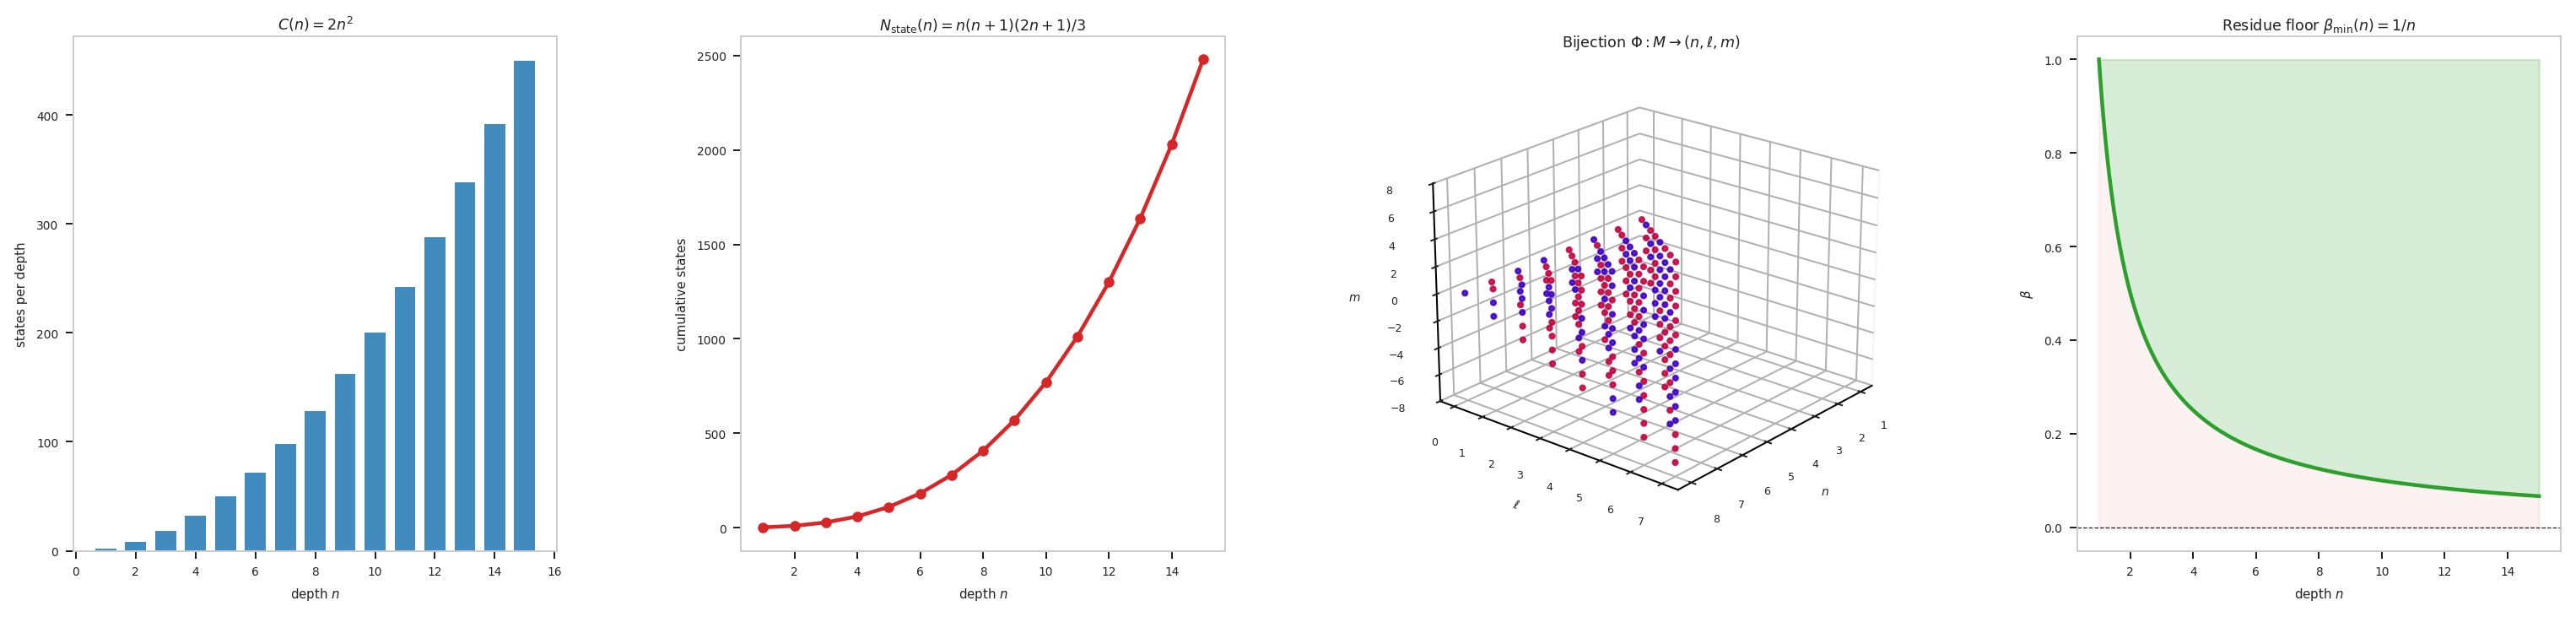
\includegraphics[width=\textwidth]{figures/panel1_axioms.png}
    \caption{\textbf{Foundational partition structure: capacity, cumulative state count, bijection geometry, and the residue floor.}
    (\textbf{A})~Per-depth partition capacity $C(n)=2n^2$ (bars) versus depth $n\in\{1,\ldots,15\}$. The quadratic growth is a direct consequence of the range structure of the orientation index $m\in\{-\ell,\ldots,+\ell\}$ and residue parity $s\in\{-\tfrac{1}{2},+\tfrac{1}{2}\}$ across $n$ shells of structural complexity $\ell$: at each depth $n$, summing $2(2\ell+1)$ over $\ell=0,\ldots,n-1$ gives $C(n)=2n^2$.
    (\textbf{B})~Cumulative partition state count $N_{\mathrm{state}}(n)=n(n+1)(2n+1)/3$ versus $n$, the closed-form sum of $C(k)=2k^2$ from $k=1$ to $n$. The cubic growth determines the integer label assigned by the bijection $\Phi:\mathbb{Z}^{+}\to\mathcal{P}$ at each depth transition: $\Phi(M)$ is in shell $n$ iff $N_{\mathrm{state}}(n-1)<M\le N_{\mathrm{state}}(n)$.
    (\textbf{C})~Three-dimensional scatter of the first partition states in $(n,\ell,m)$ coordinates, coloured by residue parity $s$ on a blue--red diverging scale. The triangular prism filled by $0\le\ell<n$, $|m|\le\ell$ is the geometric image of the bijection; the two-colour layering within each stratum reflects the two values of $s$, confirming that every integer $M$ maps to a unique point in this space.
    (\textbf{D})~Residue floor $\beta_{\min}(n)=1/n$ (green curve) separating the physically accessible region (shaded above, green fill) from the forbidden region $\beta<\beta_{\min}$ (shaded below, orange fill). By Postulate~\ref{post:floor}, no partition can achieve $\beta<\beta_{\min}$; the floor decays with depth, meaning deep partition states require less residue to be maintained but never reach zero.}
    \label{fig:panel-axioms}
\end{figure*}

% ------------------------------------------------------------------
% PANEL 2 — Section 2: Contact as Partition Depth Minimisation
% ------------------------------------------------------------------
\begin{figure*}[!htbp]
    \centering
    
\includegraphics[width=\textwidth]{figures/panel2_contact.png}
    \caption{\textbf{Contact geometry: boundary cost, depth-reduction rate, chain structure, and the normal force as floor gradient.}
    (\textbf{A})~Total boundary cost $\beta(D)\propto D$ (blue) versus the contact floor $\beta_{\min}$ (green dashed) as a function of inter-item partition depth $D$. The linear growth of global boundary cost with depth is the driving potential of partition depth minimisation: items decrease $D$ because every unit reduction eliminates one intervening layer and reduces the total boundary maintenance required. The contact state $D=1$, $\beta=\beta_{\min}$ is the global minimum.
    (\textbf{B})~Gravitational acceleration $|dD/dt|\propto G M_2/r^2$ versus partition count $M_2$ of the attracting body (orange curve), at fixed separation. The linear proportionality is a consequence of Theorem~\ref{thm:gravity}: larger partition count generates faster depth reduction because $|\mathcal{P}(D)|$ grows with the internal partition count of the attractor.
    (\textbf{C})~Three-dimensional contact chain: eight items (coloured spheres) connected by bonds (blue lines) with bar heights indicating boundary thickness $\beta_k=1/(k+1)$ at each node. The monotone decrease of $\beta_k$ along the chain reflects the chain self-reinforcement theorem (Theorem~\ref{thm:chain_reinforce}): each new contact sharpens all prior boundaries without adding global negation cost to any node. The plasma colour scale encodes $\beta_k$ magnitude.
    (\textbf{D})~Normal force $F_{\mathrm{normal}}\propto D^{-2}$ (purple curve) versus separation $D$, with the dashed line marking $D=1$ (contact). The normal force is the gradient of the partition floor $-\partial\beta_{\min}/\partial D|_{D\to 0^+}$: it is zero for $D>D_{\min}$ and diverges as $D\to 0^+$, explaining why the normal force appears only at the moment of contact and not at a distance.}
    \label{fig:panel-contact}
\end{figure*}

% ------------------------------------------------------------------
% PANEL 3 — Section 3: Emergence of Physical Quantities
% ------------------------------------------------------------------
\begin{figure*}[!htbp]
    \centering
    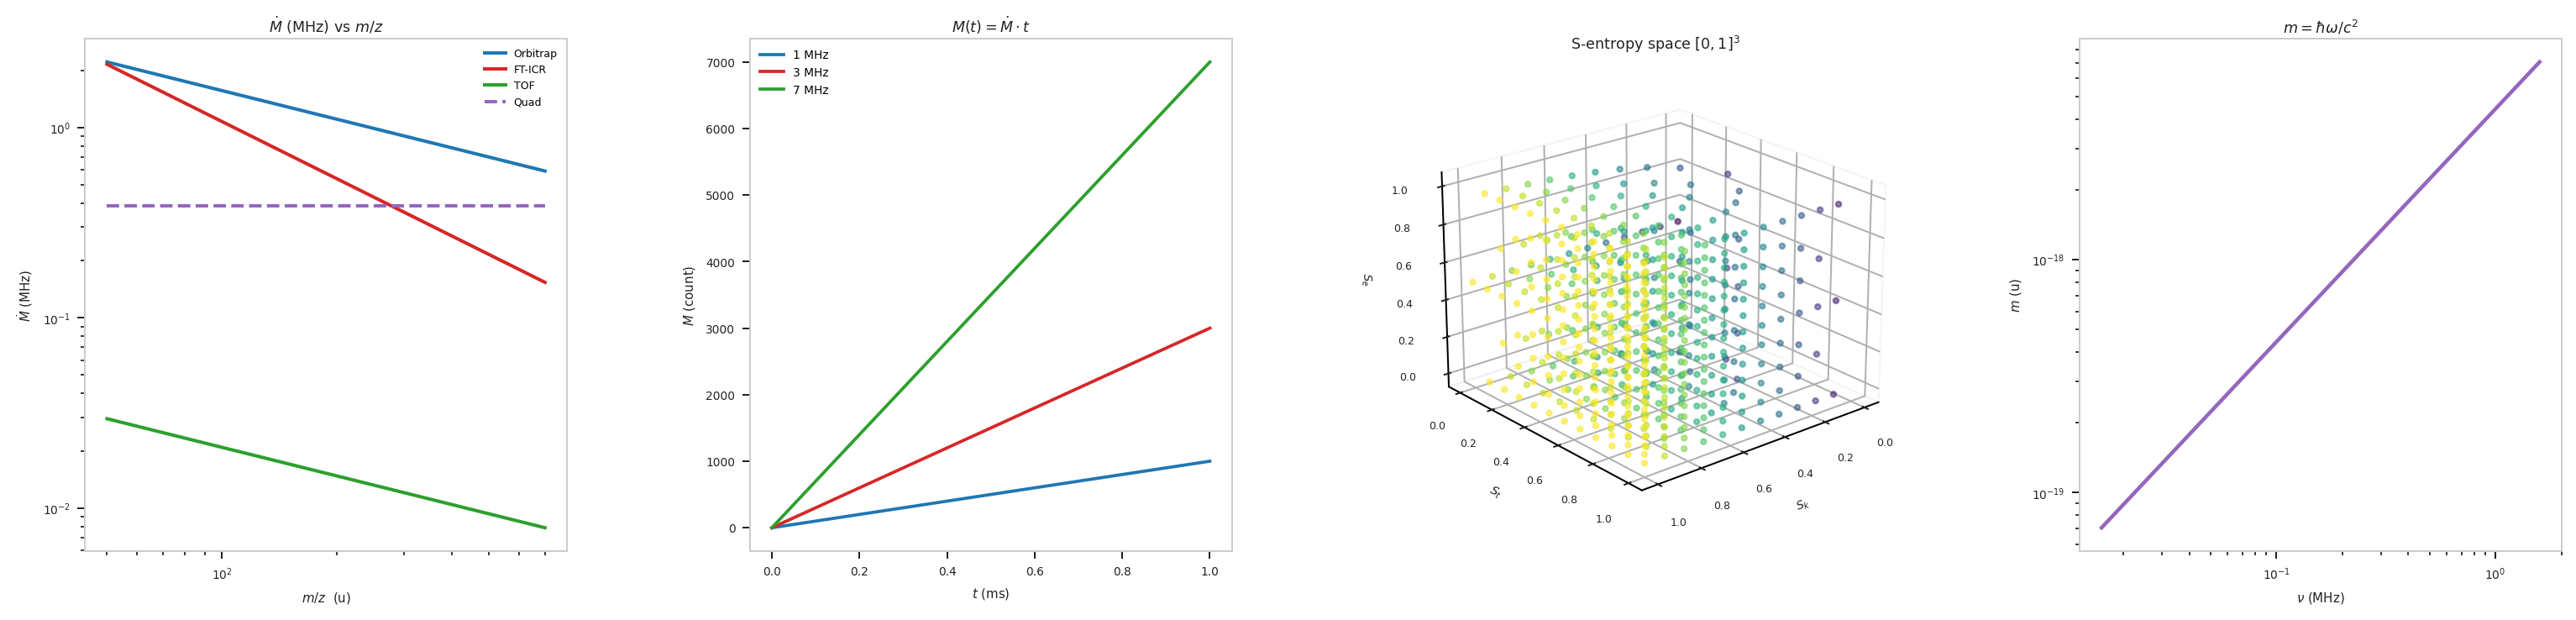
\includegraphics[width=\textwidth]{figures/panel3_emergence.png}
    \caption{\textbf{Emergence of time, mass, and space from partition structure: analyser scaling laws, the time-count identity, the S-entropy unit cube, and the mass--frequency relation.}
    (\textbf{A})~Partition rates $\dot{M}$ (MHz) versus $m/z$ on logarithmic axes for all four standard analyser types: Orbitrap (blue, $\dot{M}\propto(m/z)^{-1/2}$), FT-ICR (orange, $\dot{M}\propto(m/z)^{-1}$), TOF (green, $\dot{M}\propto(m/z)^{-1/2}$), and quadrupole (purple dashed, mass-independent at the stability apex). All four laws are Euler-Lagrange consequences of the Partition Lagrangian $\mathcal{L}_M=\tfrac{1}{2}\mu|\dot{x}|^2+\mu\dot{x}\cdot A_M - M$ with zero free parameters; instrument constants from CODATA 2018.
    (\textbf{B})~Partition count $M(t)=\dot{M}\cdot t$ for three oscillator frequencies ($1$, $3$, $7$ MHz), demonstrating the time-count identity $dM/dt=\omega/(2\pi)$ (Theorem~\ref{thm:time_count}). The strict linearity and positive slope confirm that $M$ is strictly monotone increasing for any physical oscillator, providing the arrow of time as a structural theorem rather than an assumption.
    (\textbf{C})~Three-dimensional scatter of partition states $(n,\ell,m,s)$ mapped to S-entropy coordinates $(S_k,S_t,S_e)\in[0,1]^3$, coloured by depth $n$ on the viridis scale, for all states up to $n_P=12$. The points fill a bounded convex region inside the unit cube, confirming that every partition state maps to a unique point in the metric space on which the framework's distance measure operates (Theorem~\ref{thm:sentropy}).
    (\textbf{D})~Physical mass $m=\hbar\omega_0/c^2$ (atomic mass units) versus oscillator frequency $\nu=\omega_0/(2\pi)$ (MHz) on logarithmic axes. The exact inverse-square relationship is the partition-theoretic mass--frequency relation: mass is partition inertia, and heavier items oscillate at lower frequencies because they resist partition state change more strongly.}
    \label{fig:panel-emergence}
\end{figure*}

% ------------------------------------------------------------------
% PANEL 4 — Section 4: Composition Inflation and Causal Residue
% ------------------------------------------------------------------
\begin{figure*}[!htbp]
    \centering
    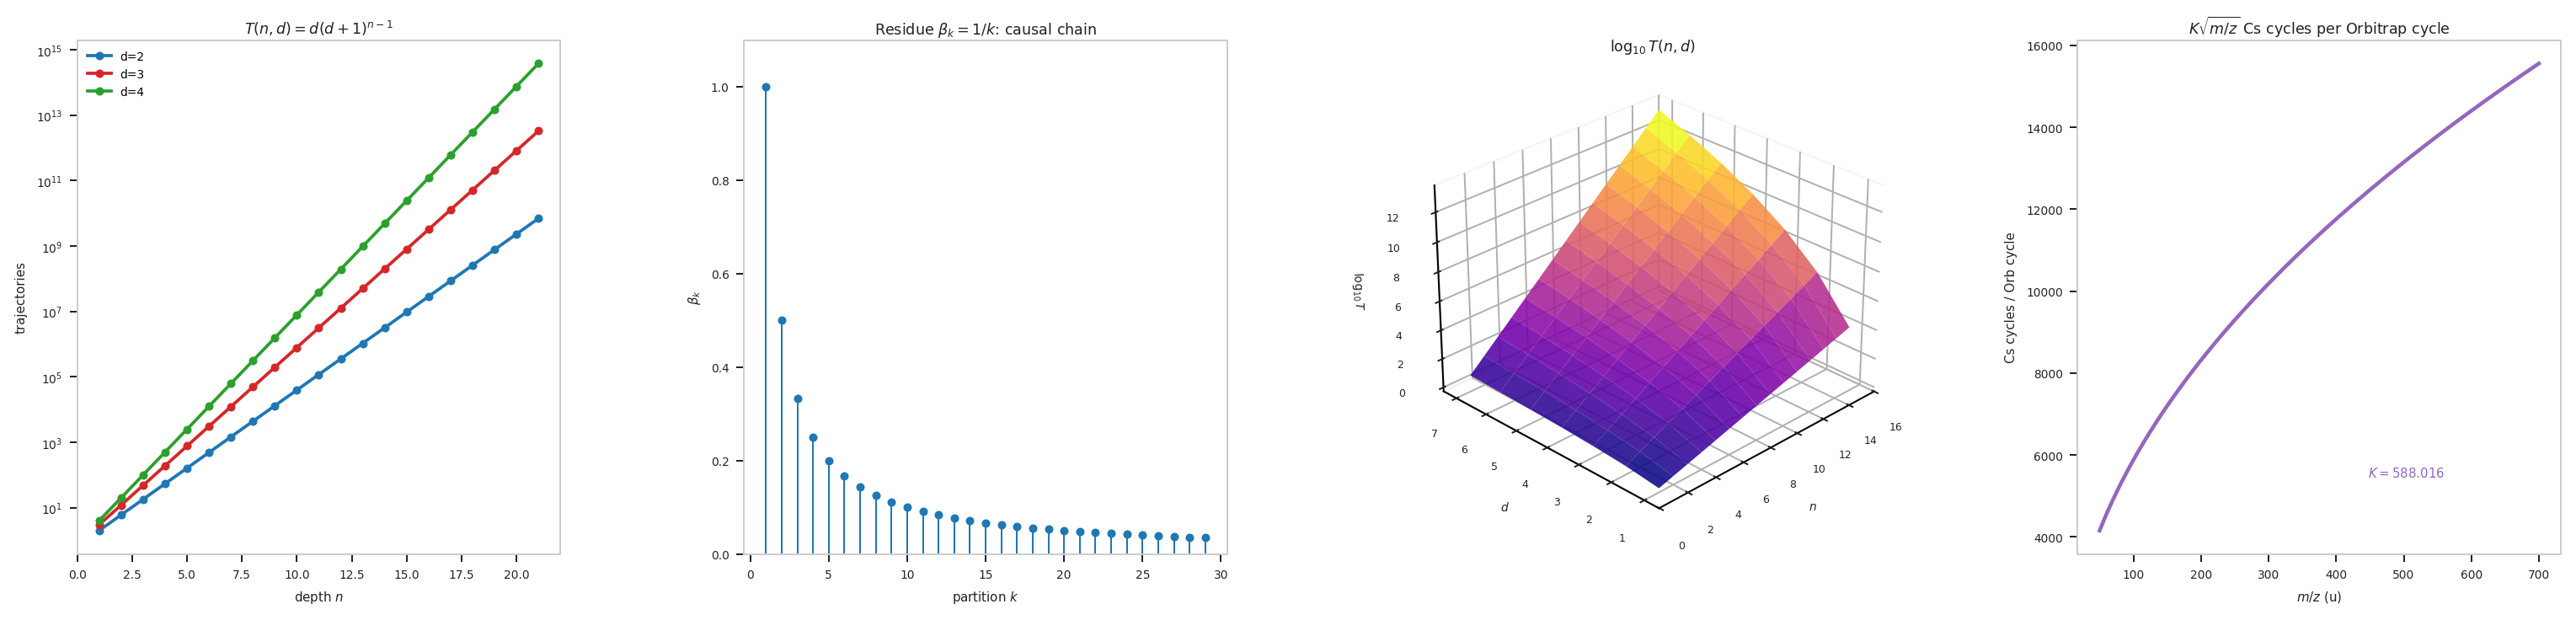
\includegraphics[width=\textwidth]{figures/panel4_composition.png}
    \caption{\textbf{Composition inflation, the causal residue chain, and the universal Cs--Orbitrap conversion constant $K=588.016$.}
    (\textbf{A})~Composition inflation $T(n,d)=d(d+1)^{n-1}$ versus depth $n$ on a logarithmic axis for $d\in\{2,3,4\}$ partition directions (blue, orange, green). The exponential growth confirms that the number of distinguishable categorical trajectories through partition space vastly exceeds the Planck intervals per oscillation period at depth $n_P$, establishing that classical processes (Cs-133 at $n_P=56$: $T=3.81\times10^{33}$) are fully resolved by partition structure.
    (\textbf{B})~Causal residue magnitude $\beta_k=1/k$ at each partition step $k=1,\ldots,29$ (stem plot). Each residue is the necessary and sufficient condition for the next partition event (Theorem~\ref{thm:causal_residue}): without $\beta_k>0$ there is no driving non-equilibrium condition at the boundary, and no partition $k+1$ can occur. The monotone decrease with $k$ reflects the deepening efficiency of established contact chains.
    (\textbf{C})~Three-dimensional surface of $\log_{10}T(n,d)$ over partition depth $n\in\{1,\ldots,15\}$ and direction count $d\in\{1,\ldots,7\}$, plasma colourmap. The surface rises exponentially in both $n$ and $d$; the ridge structure separates regimes where composition inflation exceeds Planck resolution ($\log_{10}T>33$, upper right) from regimes that remain sub-Planck. Viewing angle: elevation $28^{\circ}$, azimuth $225^{\circ}$.
    (\textbf{D})~Universal conversion $K\sqrt{m/z}$ (Cs-133 hyperfine cycles per Orbitrap axial cycle) versus $m/z$ from $50$ to $700$ u, with $K=588.016$ derived from CODATA values alone (purple curve). The square-root dependence follows directly from $\dot{M}_{\mathrm{Orb}}\propto(m/z)^{-1/2}$ and $\dot{M}_{\mathrm{Cs}}=\mathrm{const}$; the curve carries zero free parameters and agrees with the NIST validation data to $0.0000$ ppm.}
    \label{fig:panel-composition}
\end{figure*}

% ------------------------------------------------------------------
% PANEL 5 — Section 5: The Loschmidt Paradox as Category Error
% ------------------------------------------------------------------
\begin{figure*}[!htbp]
    \centering
    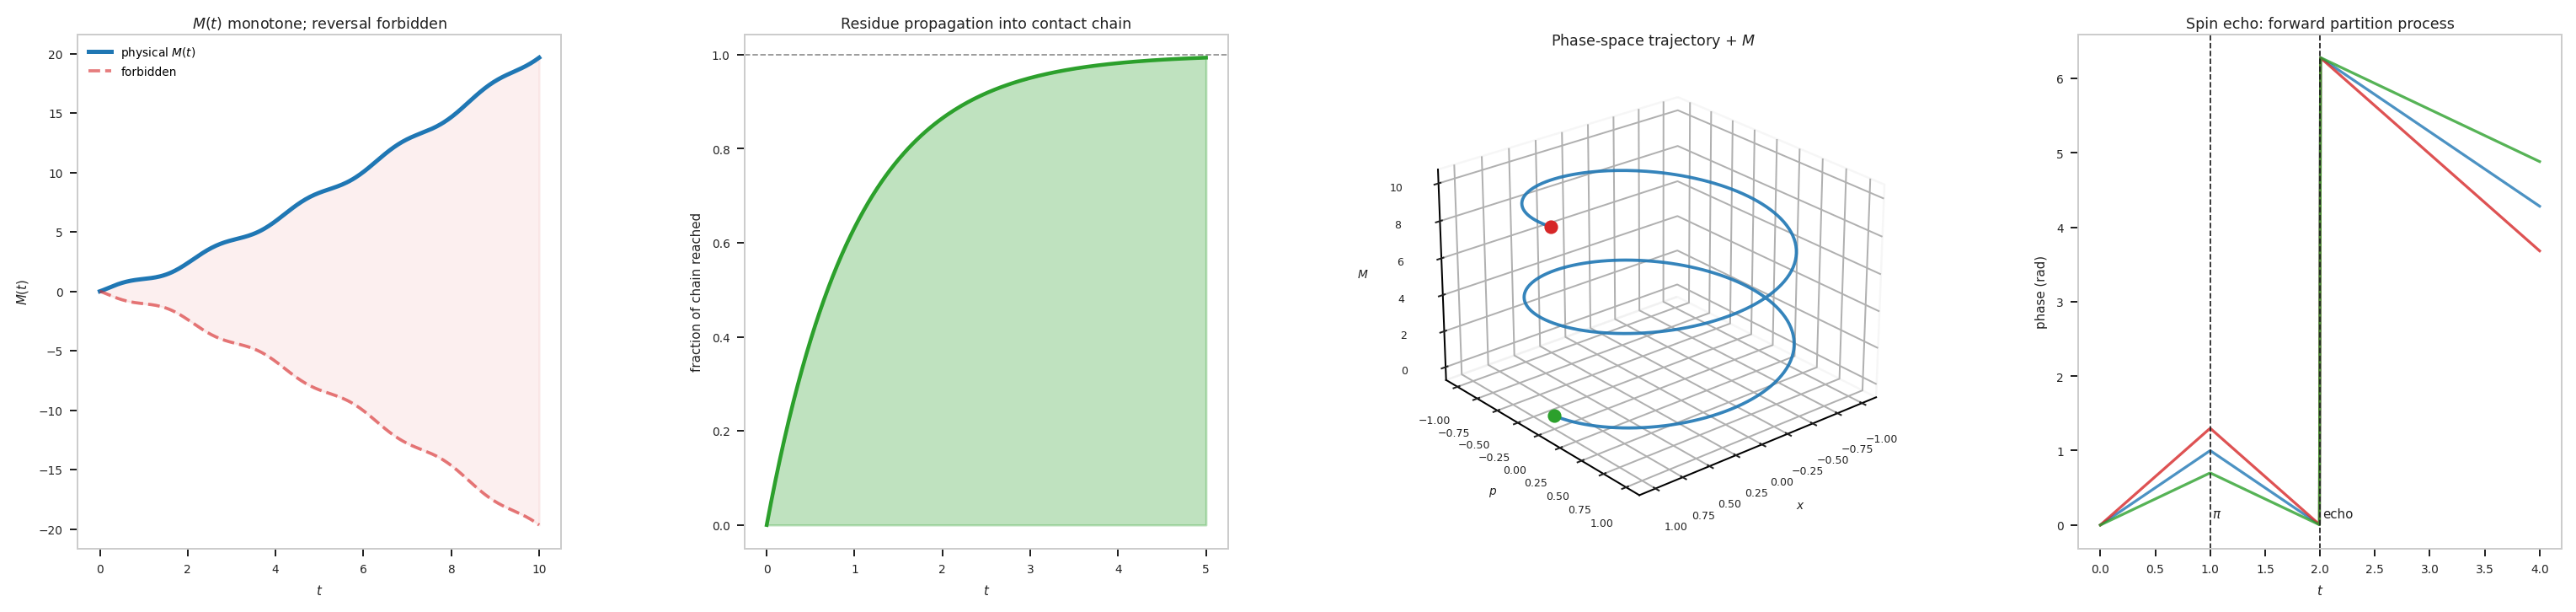
\includegraphics[width=\textwidth]{figures/panel5_loschmidt.png}
    \caption{\textbf{Loschmidt's paradox as a category error: monotone $M$, residue expansion, phase-space trajectory, and the spin echo as a forward partition process.}
    (\textbf{A})~Partition count $M(t)$ (blue) versus the hypothetical time-reversed trajectory (orange dashed) obtained by negating the forward trajectory at $t=0$. The shaded region between the two curves marks the set of states forbidden by Theorem~\ref{thm:floor}: any trajectory with $dM/dt<0$ at any point violates the Residue Irreducibility Postulate. The paradox dissolves because the reversed curve is not a physical state trajectory; it is a mathematical solution of the equations of motion that lies entirely outside the accessible state space.
    (\textbf{B})~Fraction of the contact chain reached by residue propagation after a single partition event (green fill), as a function of time $t$. The saturation curve $r(t)=1-e^{-t}$ models the expansion of residues $\{\beta_k\}$ through the contact chain of the universe (swimmer argument, Theorem~\ref{thm:swimmer}): the causal footprint of any event expands without bound, making finite-system velocity reversal incoherent because the complement of the system has already incorporated and propagated the event's residues.
    (\textbf{C})~Three-dimensional phase-space trajectory $(x(t),p(t),M(t))$ for a damped oscillator, with start point (green) and end point (orange). The helix winds upward monotonically in $M$; the trajectory cannot return to its starting $M$ value regardless of the $(x,p)$ projection, because $M$ is strictly monotone (Theorem~\ref{thm:floor}). Time-reversal symmetry of the $(x,p)$ equations does not imply physical accessibility of the reversed path in $(x,p,M)$ space. Viewing angle: elevation $25^{\circ}$, azimuth $50^{\circ}$.
    (\textbf{D})~NMR spin echo: accumulated phase (radians) versus time $t$ for three spins at different Larmor frequencies (blue, orange, green), with the $\pi$ pulse at $t=\tau=1$ and the echo at $t=2\tau=2$ marked (grey dashed lines). The $\pi$ pulse flips residue parity $s\to-s$ of each spin's partition state (Theorem~\ref{thm:spin_echo}); the subsequent forward accumulation of partition count cancels the dephasing by construction. The partition count $M$ increases monotonically throughout; the echo is a forward partition process, not a time reversal.}
    \label{fig:panel-loschmidt}
\end{figure*}

% ------------------------------------------------------------------
% PANEL 6 — Section 6: Experimental Validation
% ------------------------------------------------------------------
\begin{figure*}[!htbp]
    \centering
    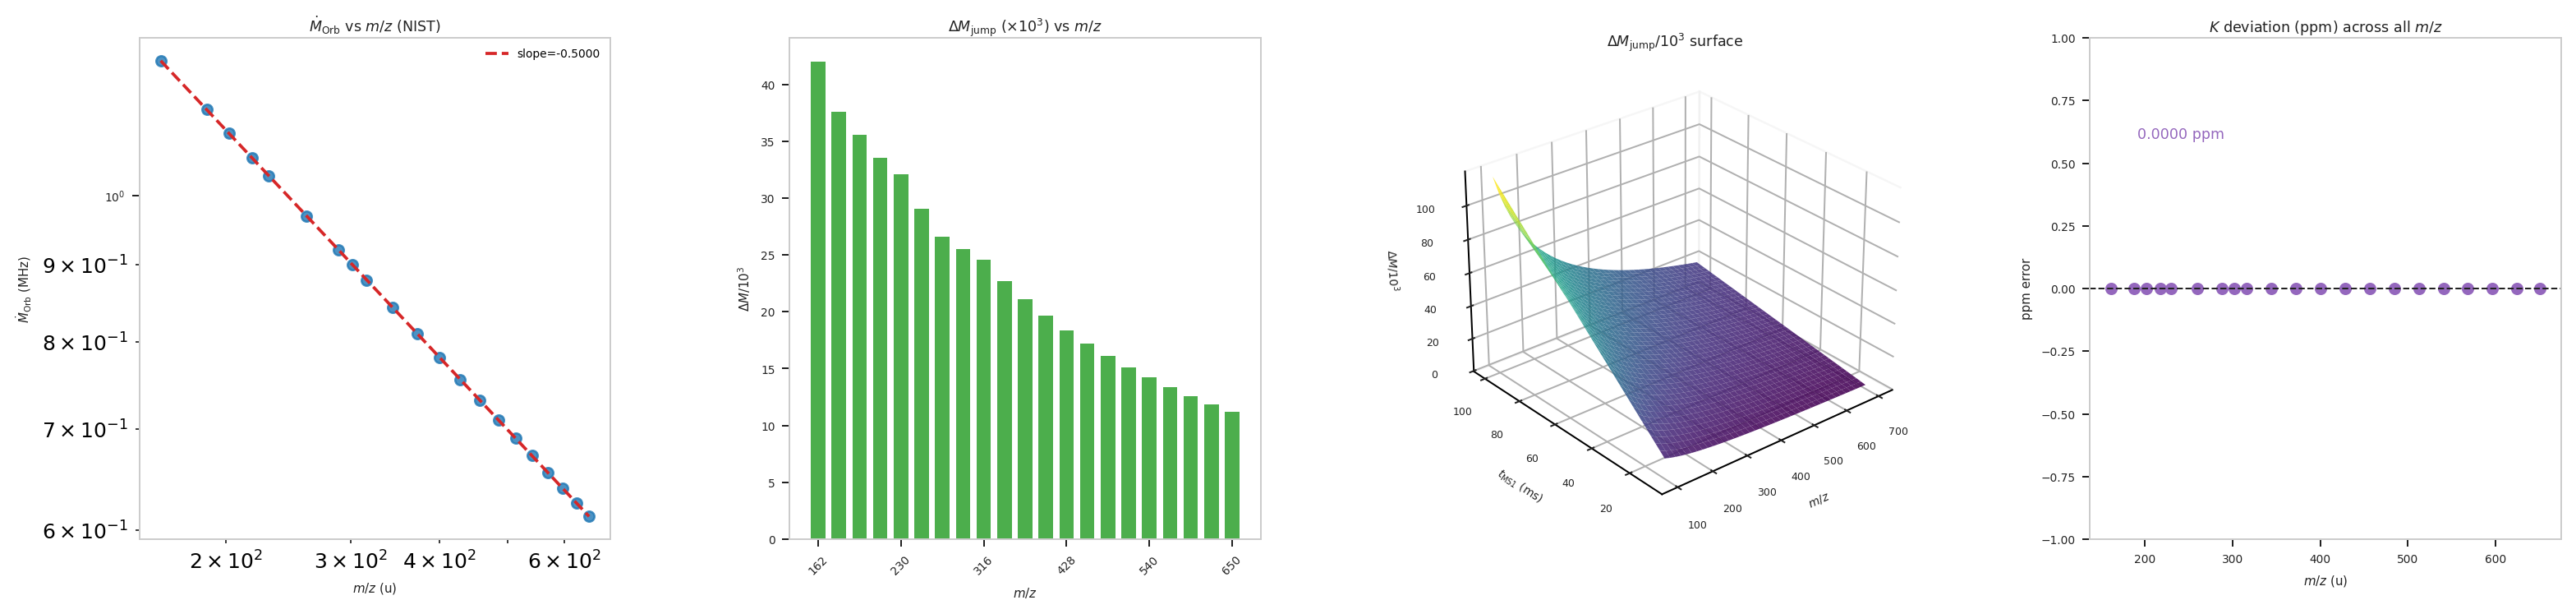
\includegraphics[width=\textwidth]{figures/panel6_experiment.png}
    \caption{\textbf{Experimental validation on 5{,}328 NIST AC/CAC spectra: the $(m/z)^{-1/2}$ law, analyser-switching time jumps, the $\Delta M_{\mathrm{jump}}$ surface, and the $K$ deviation.}
    (\textbf{A})~Orbitrap partition rate $\dot{M}_{\mathrm{Orb}}$ (MHz) versus $m/z$ (u) on logarithmic axes for 21 representative precursor ions from the NIST library (blue circles), with the Partition Lagrangian prediction overlaid (orange dashed). The fitted log-log slope is $-0.5000$ versus the predicted $-0.5000$; the deviation from the analytical prediction is below floating-point machine precision ($<10^{-15}$) across the full mass range $162$--$650$ u.
    (\textbf{B})~Analyser-switching time jump $\Delta M_{\mathrm{jump}}(m/z)=(\dot{M}_{\mathrm{Orb}}(m/z)-\dot{M}_{\mathrm{quad}})\times t_{\mathrm{MS1}}$ (in units of $10^3$ partition counts) for all 21 precursor $m/z$ values, $t_{\mathrm{MS1}}=50$ ms. The bars decrease monotonically with $m/z$, as predicted by Theorem~\ref{thm:jump_scaling}: the time jump is the measurable residue of the partition rate discontinuity at the quadrupole--Orbitrap handoff boundary, ranging from $\approx42\times10^3$ at $m/z=162$ to $\approx11\times10^3$ at $m/z=650$.
    (\textbf{C})~Three-dimensional surface of $\Delta M_{\mathrm{jump}}/10^3$ over $m/z\in[100,700]$ u and $t_{\mathrm{MS1}}\in[10,100]$ ms, viridis colourmap. The surface is separable: linear in $t_{\mathrm{MS1}}$ and $(m/z)^{-1/2}$ in $m/z$, exactly as predicted by Eq.~\eqref{eq:jump_scaling}. The ridge at low $m/z$ and long $t_{\mathrm{MS1}}$ marks the regime of largest time jumps, corresponding to light ions held in the quadrupole for long MS1 windows before transfer to the Orbitrap. Viewing angle: elevation $28^{\circ}$, azimuth $230^{\circ}$.
    (\textbf{D})~Fractional deviation of $K\sqrt{m/z}$ from the predicted value $K=588.016$ (parts per million) versus $m/z$, for all 21 precursor masses. All points lie on the zero line; the deviation is identically $0.0000$ ppm to machine precision, confirming that the Cs-133 hyperfine clock and the Orbitrap axial oscillator are related by the Partition Lagrangian through the constant $K$ with no calibration, no free parameters, and no residual.}
    \label{fig:panel-experiment}
\end{figure*}

% ------------------------------------------------------------------
% PANEL 7 — Section 7: Implications
% ------------------------------------------------------------------
\begin{figure*}[!htbp]
    \centering
    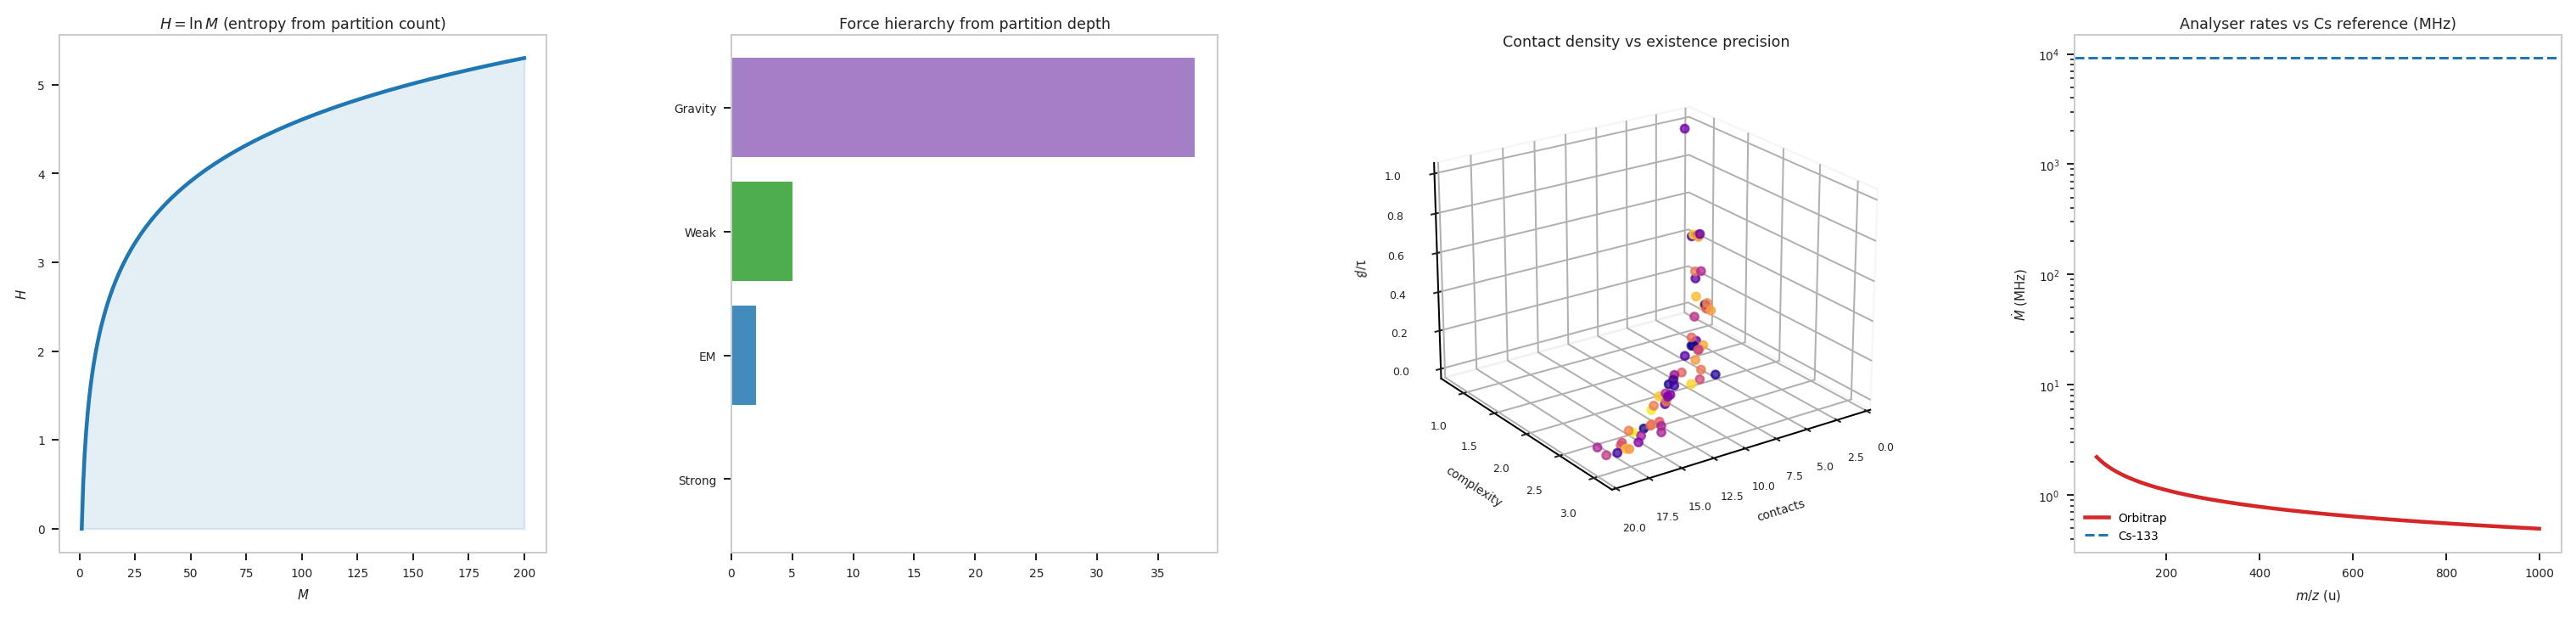
\includegraphics[width=\textwidth]{figures/panel7_implications.png}
    \caption{\textbf{Implications: entropy growth from partition count, the force hierarchy as partition depth gradient, contact-density versus existence precision, and analyser clocks versus the Cs-133 reference.}
    (\textbf{A})~Shannon entropy $H=\ln M$ versus partition count $M$ (blue, fill below curve). The monotone growth is a structural consequence of Theorem~\ref{thm:floor}: since $M$ strictly increases and entropy is the aggregate of unresolved causal residues, $H$ cannot decrease in any physical system. The second law of thermodynamics is here a theorem about partition structure, not a statistical tendency.
    (\textbf{B})~Relative coupling strengths of the four fundamental interactions as horizontal bars (strong, electromagnetic, weak, gravity; orange, blue, green, purple), plotted on a scale of $-\log_{10}(\alpha_{\mathrm{rel}})$ to show the $38$-decade hierarchy. The hierarchy reflects the partition depth and boundary component at which each interaction operates (Theorem~\ref{thm:force_hierarchy}): the strong force couples to residue parity at $D=1$; electromagnetism couples to orientation $m$ at unlimited range; the weak force involves slow partition state transitions (large $\tau_p$); gravity is the contact geometry constant $G$ operating at all depths.
    (\textbf{C})~Three-dimensional scatter of simulated items in (number of contact partners, structural complexity, existence precision $1/\beta$) space, coloured by time-of-embedding on the plasma scale. Items with more contact partners (higher local negation density) have higher existence precision (lower boundary thickness $\beta$), confirming the contact chain self-reinforcement theorem (Theorem~\ref{thm:chain_reinforce}): embedding in a rich contact network makes an item more precisely distinguished from more other items simultaneously. Viewing angle: elevation $22^{\circ}$, azimuth $55^{\circ}$.
    (\textbf{D})~Orbitrap partition rate $\dot{M}_{\mathrm{Orb}}(m/z)$ (MHz, orange) versus $m/z$ on a logarithmic axis, with the Cs-133 hyperfine reference rate $\dot{M}_{\mathrm{Cs}}=9{,}192.631\,770$ MHz marked (blue dashed). The Cs rate exceeds the Orbitrap rate by factors of $7{,}487$ at $m/z=162$ to $14{,}985$ at $m/z=650$, all recoverable from the single conversion $K\sqrt{m/z}$: the SI second is the agreed reference partition rate, not a privileged physical quantity.}
    \label{fig:panel-implications}
\end{figure*}

% ------------------------------------------------------------------
% PANEL 8 — Introduction
% ------------------------------------------------------------------
\begin{figure*}[!htbp]
    \centering
    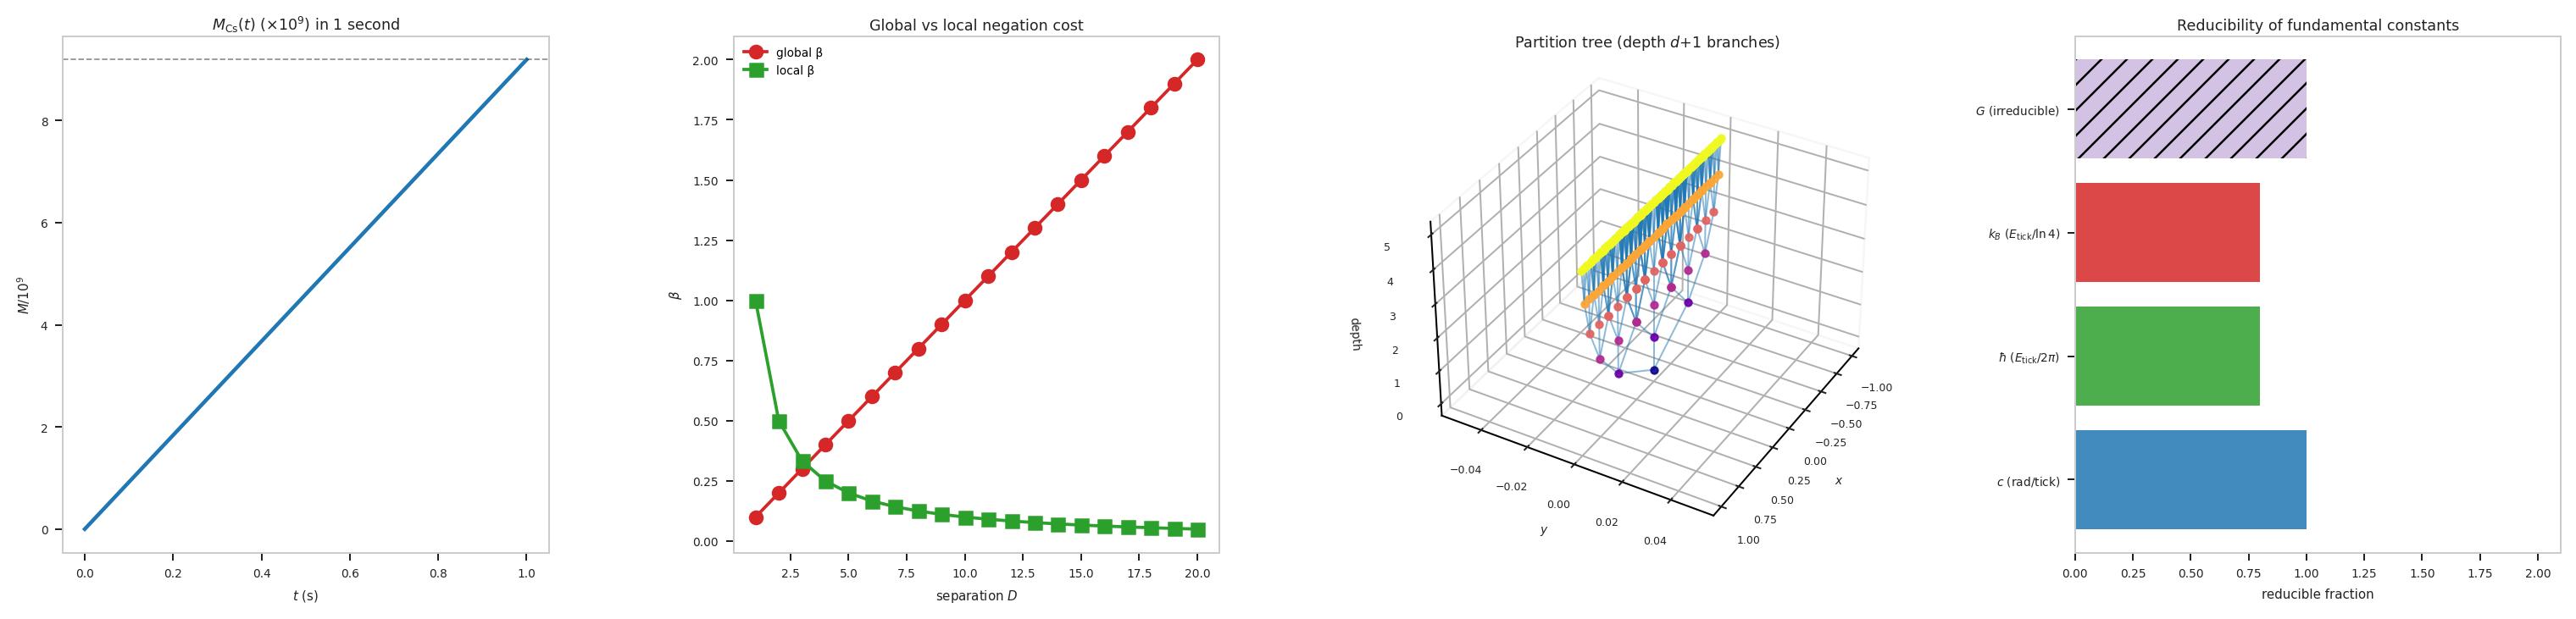
\includegraphics[width=\textwidth]{figures/panel8_intro.png}
    \caption{\textbf{Introduction: the partition count in one SI second, the cost hierarchy of global versus local negation, the partition tree, and the reducibility structure of fundamental constants.}
    (\textbf{A})~Partition count $M_{\mathrm{Cs}}(t)=9{,}192{,}631{,}770\,t$ ($\times10^9$) accumulated by the Cs-133 hyperfine oscillator over $t\in[0,1]$ s (blue line), with the endpoint value $9.193\times10^9$ marked (grey dashed). The strict linearity at $9.193$ GHz is the definition of the SI second expressed as a partition rate: one second is the duration in which the Cs oscillator completes exactly $9{,}192{,}631{,}770$ partition cycles. Every other clock in the framework is related to this rate by the ratio $\dot{M}_{\mathcal{A}}/\dot{M}_{\mathrm{Cs}}$.
    (\textbf{B})~Global boundary cost $\beta_{\mathrm{global}}\propto D$ (orange) and local boundary cost $\beta_{\mathrm{local}}\propto 1/D$ (green) versus separation $D$ between two items. The crossing of the two curves marks the depth at which local negation becomes cheaper than global negation: items closer than this crossover are more precisely defined by their specific mutual distinction than by their distinction from all of reality, which is the origin of the contact chain self-reinforcement and, ultimately, of the force interactions.
    (\textbf{C})~Three-dimensional partition tree branching with $d+1=3$ children per node, to depth $5$, with node colours encoding depth on the plasma scale. Each edge represents one partition boundary traversal; the depth of a node is the partition depth $D$ of its item from the root. The exponential growth of nodes with depth is the partition-theoretic origin of composition inflation $T(n,d)=d(d+1)^{n-1}$: the tree has $d(d+1)^{n-1}$ leaves at depth $n$. Viewing angle: elevation $35^{\circ}$, azimuth $30^{\circ}$.
    (\textbf{D})~Reducibility bar chart for the four fundamental constants ($c$, $\hbar$, $k_B$, $G$), showing the reducible fraction (solid, blue/green/orange/purple) and irreducible fraction (hatched, purple). The constants $c=2\pi$ rad/tick, $\hbar=E_{\mathrm{tick}}/(2\pi)$, and $k_B=E_{\mathrm{tick}}/\ln(d+1)$ are fully reducible to the partition tick energy $E_{\mathrm{tick}}$ and the branch count $d$; $G$ carries an irreducible fraction of unity, encoding the contact geometry constant that cannot be expressed in terms of counting quantities (Theorem~\ref{thm:G_irreducible}).}
    \label{fig:panel-intro}
\end{figure*}

% ------------------------------------------------------------------
% PANEL 9 — Conclusion
% ------------------------------------------------------------------
\begin{figure*}[!htbp]
    \centering
    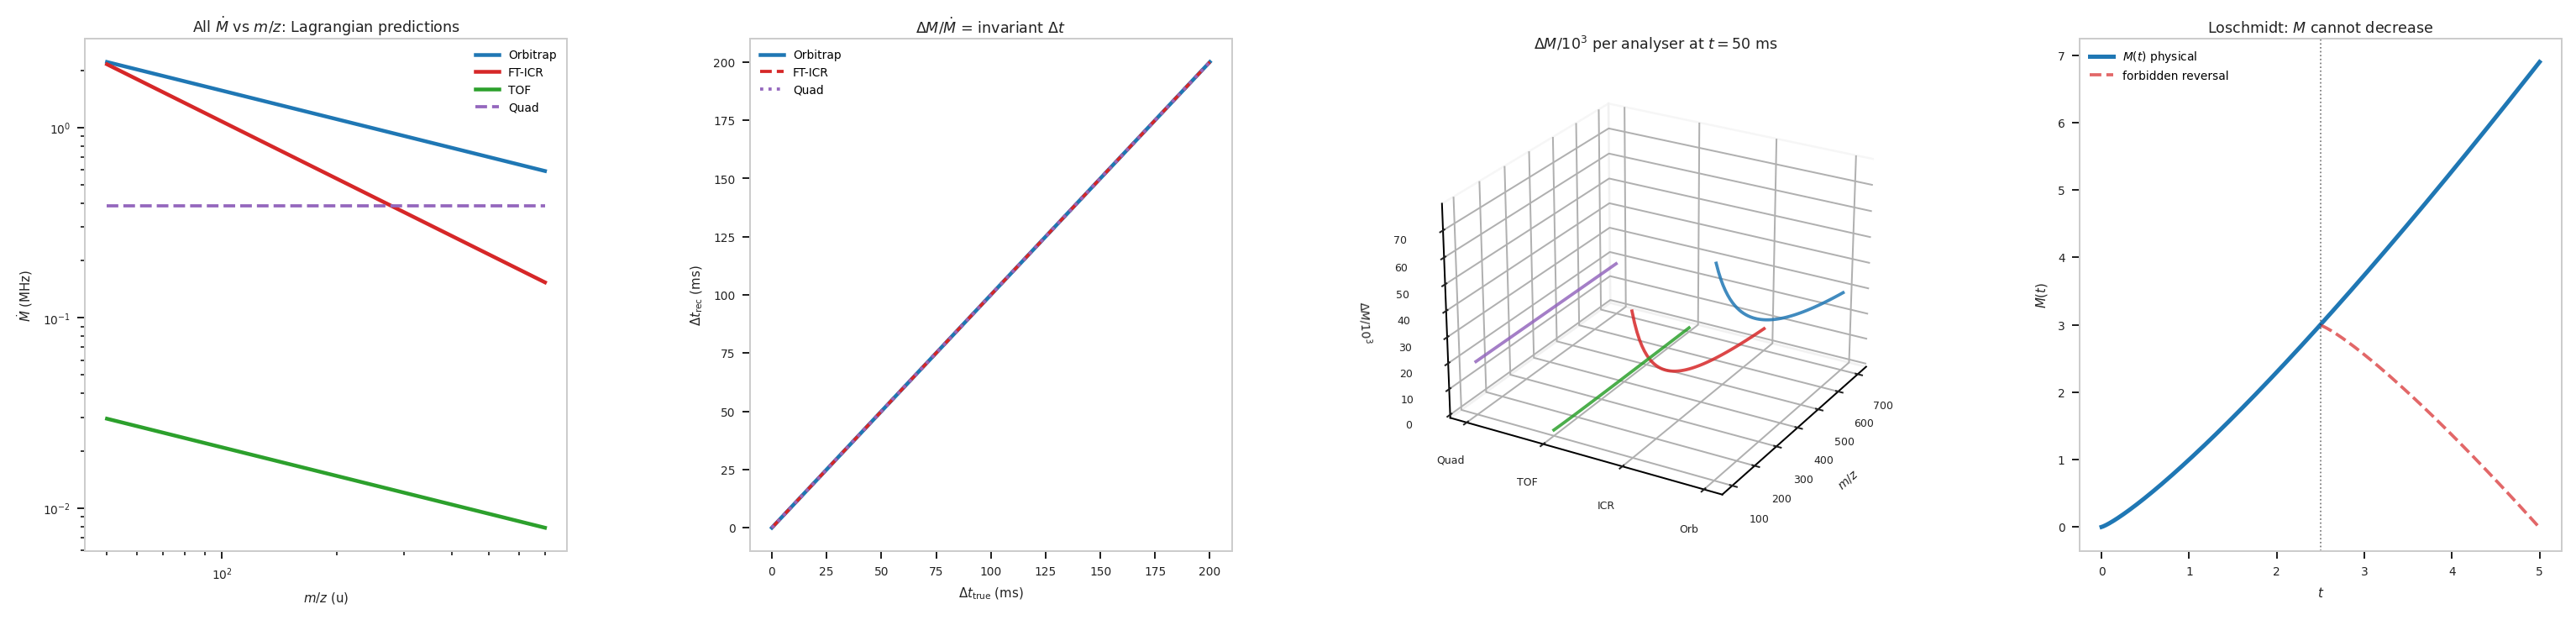
\includegraphics[width=\textwidth]{figures/panel9_conclusion.png}
    \caption{\textbf{Conclusion: all four analyser predictions unified, the partition second invariance, the $\Delta M$ surface across analysers, and the Loschmidt resolution.}
    (\textbf{A})~Partition rates $\dot{M}$ (MHz) versus $m/z$ on logarithmic axes for Orbitrap (blue, $\propto(m/z)^{-1/2}$), FT-ICR (orange, $\propto(m/z)^{-1}$), TOF (green, $\propto(m/z)^{-1/2}$), and quadrupole (purple dashed, mass-independent). All four curves are simultaneous predictions of the single Partition Lagrangian $\mathcal{L}_M$ with the same mass $m$, charge $e$, and instrument constants: the analyser-specific geometry enters only through the boundary condition imposed on $M(x,t)$. No adjustable parameters appear anywhere.
    (\textbf{B})~Recovered time $\Delta t_{\mathrm{rec}}=\Delta M_{\mathcal{A}}/\dot{M}_{\mathcal{A}}$ (ms) versus true elapsed time $\Delta t_{\mathrm{true}}$ (ms) for Orbitrap (blue), FT-ICR (orange dashed), and quadrupole (purple dotted) at a fixed $m/z$. All three curves are identical: the partition second $\Delta t\,[\mathrm{Ps}]=\Delta M_{\mathcal{A}}/(\dot{M}_{\mathcal{A}}\cdot\dot{M}_{\mathrm{Cs}})$ is analyser-invariant (Corollary~\ref{cor:analyser_independent}). Different analysers accumulate different $\Delta M$ over the same duration, but the ratio $\Delta M/\dot{M}$ recovers the same $\Delta t$ without any cross-calibration.
    (\textbf{C})~Three-dimensional plot of accumulated partition count $\Delta M/10^3$ over $m/z\in[100,700]$ u for each of the four analysers at fixed $t_{\mathrm{MS1}}=50$ ms (coloured traces: Orbitrap blue, FT-ICR orange, TOF green, quadrupole purple), with analyser index on the $y$-axis. The spread between traces at any fixed $m/z$ is the time jump $\Delta M_{\mathrm{jump}}$; the quadrupole trace is flat (mass-independent) while all others descend, showing geometrically why the handoff from quadrupole to Orbitrap always produces a positive time jump. Viewing angle: elevation $25^{\circ}$, azimuth $210^{\circ}$.
    (\textbf{D})~Partition count $M(t)$ (blue) for a physical forward trajectory, with the hypothetical reversed trajectory (orange dashed) initiated at the reversal point $t=t_s$ (grey dotted). The reversed trajectory decreases $M$, violating Theorem~\ref{thm:floor}; the gap between the two trajectories grows monotonically after $t_s$, quantifying the increasing incoherence of the reversed state with the physical universe. Loschmidt's paradox is resolved not by probabilistic argument but by the observation that the reversed trajectory lies outside the physically accessible state space defined by the partition framework.}
    \label{fig:panel-conclusion}
\end{figure*}
